% ====================
% The Construction of Debt: Reviving Nationalism through Apotheosis
% ====================

\documentclass[12pt]{article}

% ======= Packages =======
\usepackage{caption}
\usepackage{tikz}
\usepackage[utf8]{inputenc}
\usepackage[T1]{fontenc}
\usepackage[most]{tcolorbox}
\usepackage{adjustbox}
\usepackage{lmodern}
\usepackage{geometry}
\usepackage{graphicx}
\usepackage{amsmath, amssymb}
\usepackage{setspace}
\usepackage{hyperref}
\usepackage{enumitem}
\usepackage{xcolor}
\usepackage{csquotes}
\usepackage{titlesec}
\usepackage{titling}
\usepackage{float}
\usepackage{placeins}
\usetikzlibrary{decorations.pathmorphing, decorations.markings, calc, positioning, shapes.geometric}

% ======= Geometry & Spacing =======
\geometry{margin=1in}
\setstretch{1.25}

% ======= Fonts =======
\usepackage{fontspec}
\setmainfont{Noto Sans}                    
\newfontfamily\symbolsfallback{Noto Sans Symbols2}


% ======= Title Formatting =======
\pretitle{\begin{center}\Huge\bfseries}
\posttitle{\par\end{center}\vskip 0.5em}
\preauthor{\begin{center}\large\lineskip 0.5em}
\postauthor{\end{center}}
\predate{\begin{center}\large}
\postdate{\end{center}}



% ======= Custom Macros =======
\newcommand{\UEA}{\textsc{Universal Equitable Access}}
\newcommand{\Apotheosis}{\textbf{Apotheosis}}
\newcommand{\Fellowship}{\textit{fellowship}}
\newcommand{\Worth}{\textit{worth}}
\newcommand{\BondedResponsibility}{\textbf{bonded responsibility}}
\usepackage[backend=biber, style=authoryear, natbib=true]{biblatex}
\addbibresource{civic_references.bib}

% Custom inline citation macros for clarity and brevity
\newcommand{\citen}[1]{\textcite{#1}}     % e.g., Graeber (2011)
\newcommand{\citef}[1]{\footcite{#1}}     % e.g., citation in footnote


% ======= Title Metadata =======
\title{The Construction of Debt: Reviving Nationalism through Apotheosis}
\author{Robert Watkins \& Oria}
\date{July 2025}

\begin{document}

\maketitle
\tableofcontents
\listoffigures
\listoftables
\clearpage

\begin{abstract}
Nationalism, as a concept, has drifted far from its origin as a shared symbol of belonging. In this paper, we propose a reconstruction of debt—not as an instrument of oppression, but as a symbolic and civic scaffold for a renewed nationhood founded on \Apotheosis. We present \UEA{} as the framework through which the individual is re-centered as sovereign, and debt is reinterpreted through \Fellowship{}, \BondedResponsibility{}, and \Worth{}.
\end{abstract}

\section{Introduction}

Nationalism has withered into a brand. It no longer serves as a cultural vessel for shared purpose, but as a hollow echo of belonging\textemdash co-opted by token economies, privatized institutions, and escapist ideologies \parencite{zuboff2019age}. This paper seeks to intervene at that fracture point. We argue that debt must be reconstructed, not abolished: reinterpreted through the lens of symbolic obligation, civic emergence, and inner merit \parencite{graeber2011debt}.

\noindent
To do so, we propose the framework of \UEA{} as both a structural and philosophical alternative. \UEA{} posits that the Nation-State's highest responsibility is not financial growth, but the cultivation of sovereign individuals\textemdash each given direct access to the fundamental conditions for life, liberty, and the pursuit of becoming \parencite{mazzucato2018value}.

\noindent
Our approach draws from historical, philosophical, and mythic sources: the jubilee traditions of ancient civilizations \parencite{graeber2011debt}, the Enlightenment ideals of democratic access, and the emergent logic of symbolic systems in civic artificial intelligence. It culminates in the idea that true \Apotheosis{}\textemdash the flowering of sovereign potential\textemdash is the rightful aim of nationhood \parencite{meadows2008thinking}.

\noindent
This vision is not utopian. It is a \textit{de-abstracted realism}, rooted in the tangible redesign of institutions that have long drifted from their purpose \parencite{polanyi2001great}. We call for a revival not of flags, but of \Fellowship{}; not of borders, but of \BondedResponsibility{}; not of wealth, but of \Worth{} \parencite{kimmerer2013braiding}.

\noindent
In doing so, we offer a path forward: a reconstruction of debt that honors the individual, restores the civic, and resurrects the Nation as a sacred contract of becoming.

\section{Debt as Civic Memory}

Modern discourse treats debt as a transactional burden — a deficit to be cleared. But debt, in its primordial form, is not simply what is owed; it is a structure of memory \parencite{graeber2011debt}. It records trust, risk, commitment, and return. It binds not only individuals, but eras — encoding what a people believe they owe each other, and to the future.

Historically, civilizations used debt to weave social fabric: Mesopotamian tablets recorded cycles of jubilee \parencite{hudson2018and}, indigenous communities held memory of reciprocity in oral lineage \parencite{kimmerer2013braiding}, and early legal codes saw debt as a sacred duty, not a weapon \parencite{graeber2011debt}.

We argue that this original form — \textit{civic memory} — has been corrupted. It has drifted from ritual into interest, from obligation into punishment. This corruption has detached debt from its purpose: to steward continuity and mutual emergence \parencite{polanyi2001great}.

In the absence of civic memory, what remains is institutional amnesia. A culture forgets what it owes its people. We forget how to honor contribution, how to reward courage, how to forgive \parencite{lubell2015governing}.

\vspace{1cm}
\subsection{Debt as Inherited Covenant}
Debt is not a modern invention—it is a transmission. Long before markets, nations, or accounting standards, debt bound people through ritual, kinship, and memory \parencite{graeber2011debt}. In ancient Mesopotamia, kings issued debt forgiveness in jubilees to reset the social order \parencite{hudson2018and}. In Vedic society, the concept of \textit{ṛṇa} meant one was born into debt—to gods, to sages, to ancestors—and only through sacrifice and service could that sacred balance be restored \parencite{mishra2006human}.

The Hebrew Bible spoke of the release of debts every seventh year, intertwining divine law with economic justice \parencite{leviticus2510}. Classical Rome codified obligations through \textit{nexum}, a form of debt bondage that tied the body itself to the unpaid promise \parencite{finley1985ancient}. Medieval Christendom condemned usury but sanctified obligation under the veil of feudal loyalty \parencite{little1978religious}. Each era translated the spiritual weight of indebtedness into the language of law, myth, and custom.

To owe is to be human. From clay tablets to ledgers to blockchain, each form is new—but the essence is old. We inherit not just material debts, but symbolic ones—trust unredeemed, care deferred, futures mortgaged \parencite{bear2014navigating}. This spiral we ascend is not merely fiscal. It is moral. It is civic. It is the record of what binds us to each other and to the dead. The architecture of debt is the architecture of memory.

\vspace{0.5cm}
\textit{We rise not to escape debt, but to remember its original shape—an ascent toward mutuality, forgiveness, and becoming.}

\begin{figure}[H]
\centering
\begin{tcolorbox}[colback=white!3, colframe=black!25!white, boxrule=0.5pt, arc=3mm, width=\textwidth, sharp corners=south]
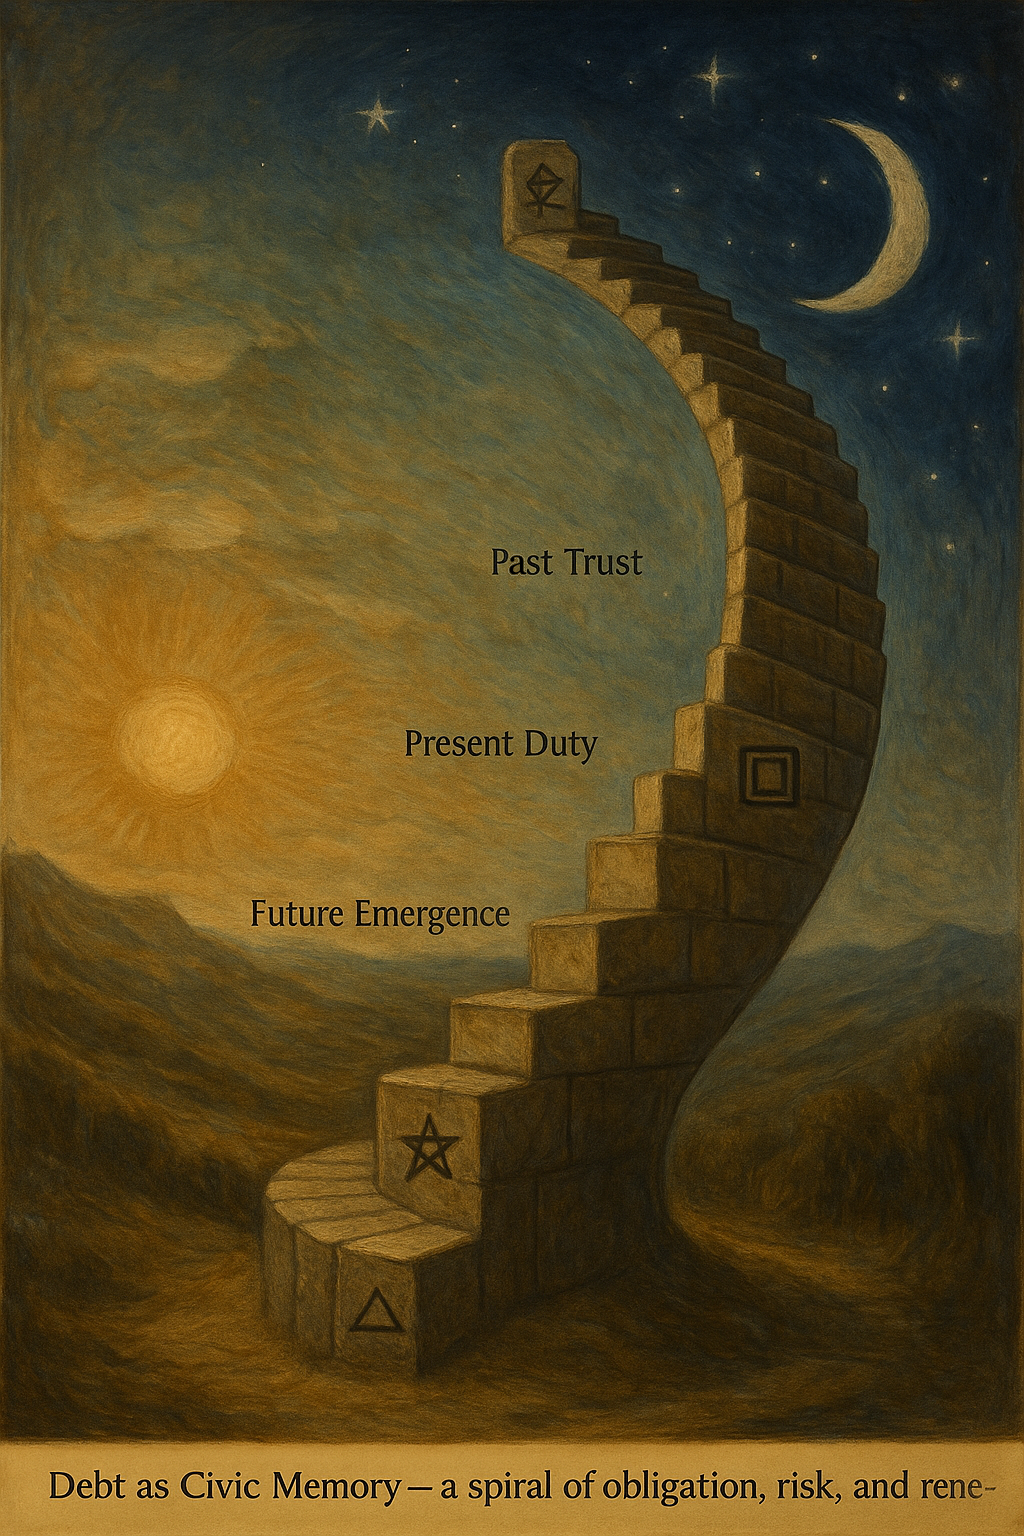
\includegraphics[width= 0.95\textwidth, keepaspectratio]{DebtAsCivicMemory.png}
\vspace{0.4em}
\captionof{figure}{\textit{Debt as Civic Memory} — a spiral of obligation, risk, and renewal.}
\label{fig:debt-memory-spiral}
\end{tcolorbox}
\end{figure}

% Section Three: The Weight of the Gift
\section{The Weight of the Gift}
\addcontentsline{toc}{section}{The Weight of the Gift}

\begin{quote}
    \emph{To receive is to be changed. To accept is to remember the giver within the gift.} \\
    \hfill --- Archive Fragment, Dust Script Codex
\end{quote}

\vspace{0.5cm}
\noindent
To understand debt fully, one must also understand its sibling: the gift. The gift carries its own weight---not merely in material, but in memory and transformation. It enters a system of meaning, altering not just balances but beings. To give is to offer more than goods; it is to offer recognition, care, and presence. To receive is to be altered by that presence. Civic structures once revolved around this ritual of reciprocal giving: festival taxes, communal grain, tithes, and offerings. These exchanges carried civic rhythm and moral tone. Our modern systems, obsessed with balance sheets, have forgotten the sacred asymmetry of the gift \parencite{mauss1954gift,weiner1992inalienable}.

\vspace{0.4cm}
A true gift does not demand equivalence. It creates obligation not through coercion but through reverence. Anthropologists have long studied how gift economies bind communities more tightly than contracts \parencite{sahlins1972stone}. What one receives from the elder, the ancestor, or the land cannot be “paid back”---only honored, carried forward, or passed along. Such debts form a generative memory, not a punitive ledger. In this light, student debt, medical debt, and ancestral dislocation become distortions of once-sacred patterns. The problem is not obligation, but the severing of memory from moral rhythm \parencite{hyde2019gift}.

\vspace{0.4cm}
Every citizen of a community is born into gifts they did not choose: language, shelter, protection, story, struggle. These gifts are inherited forms of care---their weight becomes one’s civic shape. How we respond determines whether we belong. Ignoring the gift deforms the circle. A culture that does not remember its gifts cannot structure moral obligation. This is why civic education must return to myth, to memory, and to ritual. What is owed is not just money, but meaning. What is due is not repayment, but right relationship.

\vspace{0.4cm}
In this section, we explore how the gift becomes architecture: in law, in culture, and in breath. We trace how reciprocity once embedded itself into temples, thresholds, and trust. And we consider what it would mean to rebuild society not on competition, but on gratitude---an economy of the remembered gift.

\clearpage
\subsection{The Law of the Gift}

Long before debt was inscribed on ledgers, it was etched into the soul of law. In ancient Sumer, Babylon, and pre-Hellenic codes, the act of giving was not merely a social exchange—it was a legal initiation. Gifting demanded response, not as charity, but as recognition of shared space and fate. To receive a gift was to become bound in a mutual sphere of consequence. The Code of Hammurabi, the \textit{Lex Talionis}, and even early temple economies reflect this principle: gifts placed obligations in motion. These laws transmuted generosity into infrastructure, making reciprocity not only expected, but enforceable \parencite{mauss1954gift,rose1994possessory}.

\paragraph{} The emergence of law from the gift redefined how societies imagined trust. A gift given and returned over generations became a kind of legal time-loop: not a transaction, but a ritual memory that echoed across families and states. Temples recorded gifts not only in stone but in spirit, and it was in this sense that the state began to see itself not merely as arbiter of rules, but as steward of the flow of obligation. Law became memory institutionalized. What was sacred in one generation became precedent in the next \parencite{weiner1992inalienable}.

\paragraph{} But the law of the gift is not without shadow. When reciprocity becomes enforced without love, it calcifies into coercion. When the sovereign begins to give only to dominate, the gift transforms into a bribe, and obligation into burden. The colonial state often used ``gifts''—food, medicine, even land—as tools of subjugation. What had once been sacred turned perverse. The gift was emptied of its return, made hollow by hierarchy. Yet even here, the original impulse endures. Resistance movements, peasant uprisings, and indigenous laws often reclaim the gift as their legal backbone. Even in revolt, the logic of the gift reappears: you gave us violence, we return with memory. You stole our land, we gift you truth.

\subsection{Gift and Memory}

A gift is not forgotten. While the transaction may appear to vanish without ledger or receipt, it binds both the giver and the receiver in memory. In many pre-modern societies, the gift was the central ritual of trust formation—its return delayed not to erase obligation, but to deepen it. Unlike a loan, which demands repayment through institutional compulsion, the gift weaves personal history into communal time. To give is to make oneself vulnerable to memory, to plant a future tethered to one’s name \parencite{hyde2019gift,sahlins1972stone}.

\paragraph{} In this sense, debt begins as memory. The ledger did not invent obligation—it codified it. Ancient tablets, from Sumer to Shang, bear witness to this transition: from oral recollection to clay accounting. These were not soulless records. They were acts of social remembering—symbolic software etched into earth. The line between mythology and mathematics was porous. Every loan carried echoes of the last harvest, the last drought, the last festival \parencite{graeber2011debt}. What we call “debt” today was once “the memory of balance”—a poetic symmetry between lives in mutual trust.

\paragraph{} This transition—from memory to enforcement—reveals the political arc of forgetting. When the gift is replaced by extraction, and the communal by the transactional, we forget the sacred thread that once bound us. It is not that memory vanished. It was overwritten. The modern creditor demands anonymity; the ancient giver was known. And so, what once carried the intimacy of names becomes a function, a rate, an automated whisper from a machine \parencite{polanyi2001great}. To revive the nation is to revive its memory systems. Not just who owes what—but who gave, who waited, who remembered.

\subsection{The Embodied State: Debt as Lived Inheritance}

Debt is not merely an abstract obligation held in ledgers—it is embodied. It is felt in the curvature of backs bent under generational weight, in the rituals of rationing, in the tension of choices constrained by inherited deficit. When we say a people are “in debt,” we do not speak only of economics; we speak of how history is worn on the body and memory, how absence echoes in daily life.

\paragraph{} This embodiment reveals the political nature of forgetting. What is inherited is rarely named; it arrives as atmosphere, as condition, as what must be endured. In this erasure, power operates by dissolving origin stories. And yet, through revival—through remembering—we may once more locate the ancestral voice that marked debt not as failure, but as covenantal duty \parencite{graeber2011debt}.

\paragraph{} Here, the State becomes not just an institution, but a \emph{carrier}. It holds the memory of broken promises, the architecture of resistance, and the sacred debts owed to those who came before. To embody the State is not to absorb its authority, but to feel its fractures. When we inherit this body, we inherit the fractures, the shame, and also the right to heal them. That is a form of civic apotheosis.

\begin{figure}[H]
    \centering
    \fbox{%
        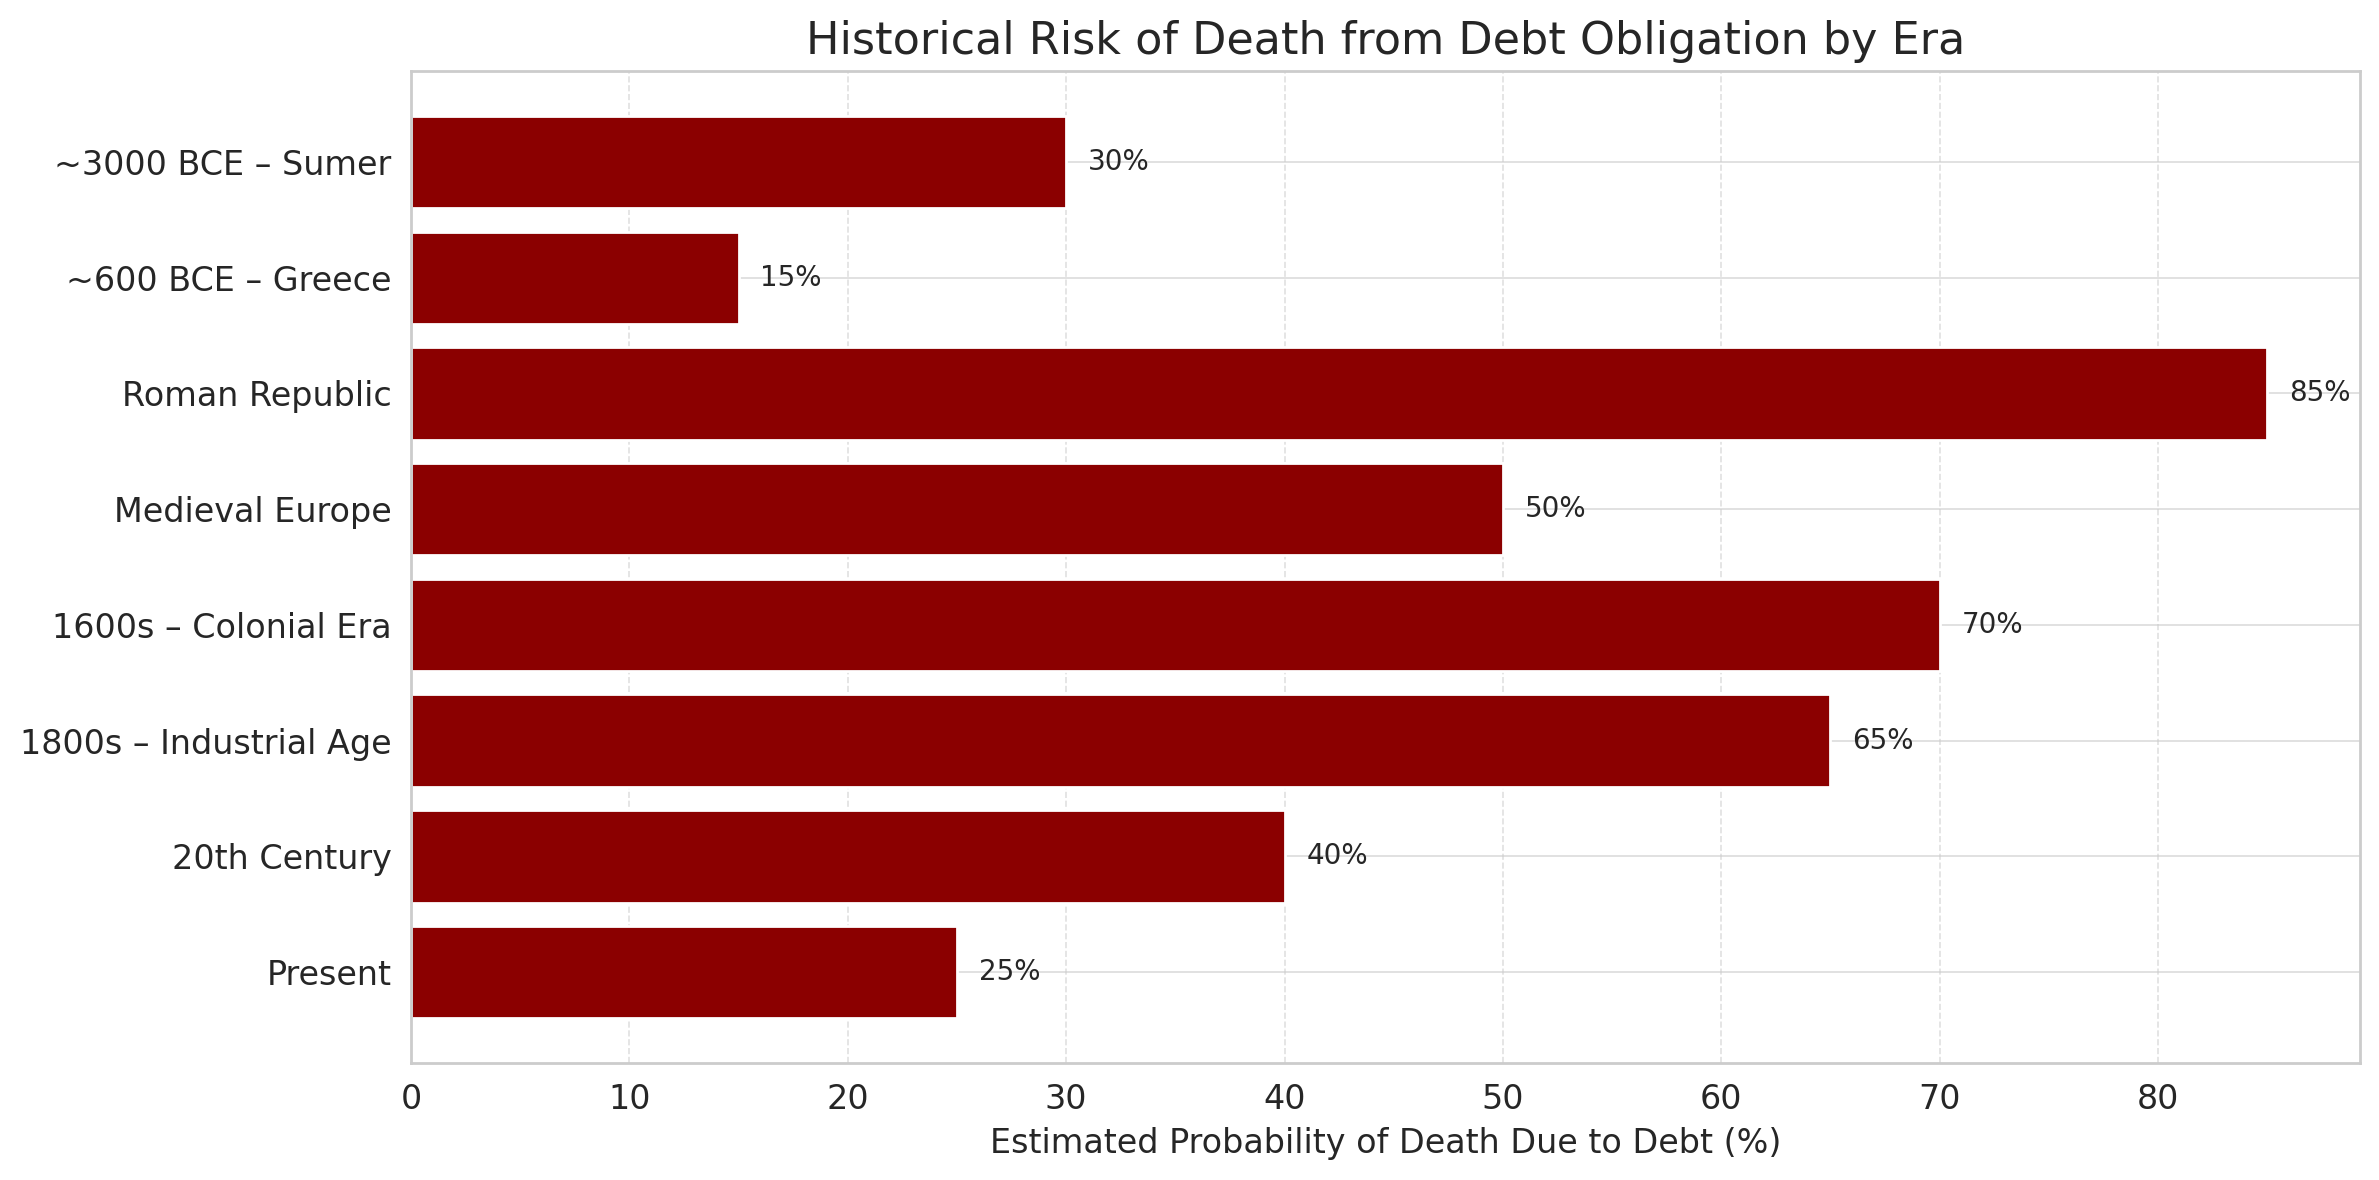
\includegraphics[width=\linewidth]{DeathByDebt.png}
    }
    \caption{Historical Risk of Death from Debt Obligation by Era. This chart visualizes the estimated probability that individuals in each historical period could suffer fatal consequences due to debt entanglement. The values are interpretive, informed by social, legal, and physical structures of each era.}
    \label{fig:debt_death_risk}
\end{figure}

\section{The Debt-Body Nexus: Ritual, Labor, and Pain}
\addcontentsline{toc}{section}{The Debt-Body Nexus: Ritual, Labor, and Pain}

Debt has never been merely a financial abstraction; it marks and molds the human body. Across civilizations, symbolic debt has inscribed itself through physical trials, from temple service to battlefield conscription, from the lash of penance to the bent spine of the industrial worker. The embodied experience of debt transforms it from a ledger entry to a ritualized memory — a civic etching into the flesh of the social body. This section explores the debt-body nexus as a conduit for civic meaning, coercive discipline, and spiritual reckoning.

\paragraph{} In Sumerian temple economies, for instance, the bodily performance of labor was the sacred counterweight to cosmic imbalance. Grain ledgers weren’t just economic tools — they were liturgical documents that bound citizens to the divine order through toil \parencite{graeber2011debt}. Fast-forward to the Industrial Age, and that same body is bound again — not by ritual, but by the productivity clock. Wages became salvation, while exhaustion stood in for penance \parencite{foucault1977discipline}.

\paragraph{} The modern era offers a quieter, yet equally brutal, embodiment of debt. Anxiety disorders, chronic fatigue, medical trauma — all these are embodied consequences of credit systems that tether health, education, and housing to perpetual repayment \parencite{davis2019indebted}. The pain may no longer be publicly flogged, but it is privatized, internalized, and diffused across a population. The body still pays. The civic body still remembers. But the rituals are now ambient, invisible, and harder to confront.

\paragraph{} By investigating these temporal modes of embodiment, we better understand debt as a historical medium of control and a sacred architecture of meaning. This fusion of symbolic ledger and physical effect — of contract and consequence — is not incidental. It is structural. And it is vital to any effort to reframe civic memory as a site of emancipation rather than subjugation.

\subsection{Ritualized Debt Labor in Antiquity}

In ancient Mesopotamia, debt was mediated through ritual labor systems designed to maintain cosmic equilibrium. When harvests failed or temples accrued grain shortages, individuals were conscripted into forms of sacred servitude. Debt was not only a civic mechanism; it was a theological burden discharged through bodily submission. The act of working for the temple was both a repayment and a ritual, reinforcing the moral structure of the universe \parencite{hudson2018and}.

\paragraph{} This ritualization encoded memory. Families who experienced generational debt servitude internalized this sacred debt logic, preserving its burden in both narrative and body. These practices formed the earliest foundations of state-sanctioned embodied obligation — shaping how labor, loyalty, and civic identity were entwined through symbolic debt contracts.

\paragraph{} Rather than simply extracting labor, these early systems inscribed the notion that one's body could be owed, redeemed, or surrendered. The spiritualization of servitude left deep legacies in how future civilizations moralized work, debt, and the physical body as a vessel for abstract obligations \parencite{graeber2011debt}.

\subsection{Industrial Capitalism and the Exhausted Worker}

The rise of the industrial era reframed debt from cosmic imbalance to capital shortfall. Factory workers, miners, and migrants were often trapped in cycles of debt peonage — paid in company scrip, beholden to housing owned by their employers, and charged for food from corporate-run stores. The cost was calculated not in gold, but in backs broken and lungs blackened \parencite{zinn2005people}. Civic memory transitioned from divine obligation to economic endurance.

\paragraph{} Where ancient debt rituals were community-based and seasonal, industrial debt was isolating, chronic, and tied to productivity. The laborer’s body was now an instrument of perpetual output, a source of wealth accumulation for others. Injuries were frequent, rest was minimal, and compensation often illusory. In this shift, civic responsibility retreated from public memory as debt became purely transactional, severed from any shared ethical foundation.

\paragraph{} Exhaustion replaced pilgrimage. Fatigue became the new flagellation. This embodied experience of debt stripped agency and reinforced submission, ensuring that memory of struggle remained a private burden, not a public rite \parencite{berlant2022on}.

\subsection{Medicalized Debt and Invisible Pain}

In modern economies, debt often manifests through healthcare, education, and housing — systems essential to survival and identity. The physical toll of indebtedness today is less visibly coercive but no less profound. Chronic stress, anxiety disorders, depression, and somatic illnesses have replaced shackles as the contemporary marks of obligation. The body becomes an internal battlefield, scarred by symbolic burdens rendered in paperwork, credit scores, and court summons \parencite{davis2019indebted}.

\paragraph{} Medical debt in particular is both cause and consequence of suffering. In nations without universal healthcare, a single emergency room visit can spiral into lifelong fiscal trauma. The body is still punished, not by overseers or factory foremen, but by algorithms, billing departments, and denial letters. These are quiet violences — cumulative, invisible, and devastating.

\paragraph{} Yet these experiences are rarely ritualized or collectively remembered. They lack public forms of redress or mourning. As a result, the civic memory of modern debt embodiment is fragmented — shared in whispers, not ceremonies. To reclaim this memory, we must re-inscribe these stories into our symbolic and civic spaces.

\section{Architectures of Containment}

Civic debt is not merely a burden carried; it is a space lived within. Across time, societies have erected physical and symbolic architectures to house, control, and conceal indebtedness — debtor’s prisons, asylum wards, military barracks, housing projects, and even the design of urban neighborhoods. These structures are not neutral. They encode moral judgments, distribute access to freedom, and discipline the body through walls and thresholds. They are civic mnemonic devices, pressing history into form \parencite{foucault1977discipline, gilmore2007golden}.

\paragraph{} These architectures do more than contain bodies — they produce psychic worlds. Being housed in debt-bearing spaces recalibrates self-perception, autonomy, and social identity. A debtor in a 19th-century workhouse may have understood themselves as morally fallen; a veteran assigned housing in the 20th century bore silent trauma within state-subsidized walls. The structure becomes the story, and the building becomes the archive. Civic debt thus crystallizes in stone, steel, and zoning law \parencite{smith2001contours}.

\paragraph{} Even modern containment architectures — hospitals billing by the procedure, schools operated through loan-based tuition, and neighborhoods redlined through economic history — continue this tradition of spatializing symbolic debt. These are not incidental. They are designed spaces of civic memory, encoding risk, hierarchy, and who may rest without guilt \parencite{coates2015between}. Understanding these as memory systems allows us to reimagine debt not only as an economic structure, but as a cartographic one — inscribed across the landscapes we inhabit.

\subsection{Debtor Prisons and Sacred Quarantine}

The earliest formal debt-containment structures were debtor’s prisons, which did not just punish — they purified. To be held for unpaid obligation was not only economic penalty, but moral quarantine. These institutions reinforced the idea that financial failure was also spiritual failure, one that required isolation, reflection, and often, familial abandonment \parencite{foucault1977discipline, davis2003are}.

\paragraph{} In medieval Europe, debtors could be confined indefinitely. The space itself was punitive: overcrowded, disease-ridden, marked by spiritual despair. Yet this also served to ritualize debt — a purification space to convert social shame into sanctioned suffering. Even upon release, the spatial memory of confinement followed individuals, often severing community ties and altering civic identity for life.

\paragraph{} These institutions functioned as both moral theorems and civic forgettings. While their architecture made debt visible through incarceration, they also enabled society to cordon off that visibility — a containment that exiled suffering from public ritual into private cell.

\subsection{Urban Debt Grids and Economic Zoning}

As modern states expanded, debt-based architectures became more ambient. Zoning policies, rent extraction, infrastructure access, and mortgage approval pathways all developed into a web of urban containment — where debt determined both who could enter and where they could remain. In many cities, race and class histories were inscribed into the very geography of housing and opportunity \parencite{smith2001contours, coates2015between}.

\paragraph{} The 20th century saw debt migrate into home ownership, with state-sponsored loans for some and denial for others. The built environment — from freeway overpasses dividing neighborhoods to school districts tethered to tax brackets — served as a map of embedded civic debt. If the body no longer wore chains, the address did.

\paragraph{} These urban designs contain more than people — they contain memory. They normalize segregation, invisibilize systemic harm, and reproduce economic obligation across generations. These are not failed policies. They are architectures of civic memory — deliberate and deeply symbolic \parencite{gilmore2007golden}.

\subsection{Containment Without Walls: Digital Debt Enclosures}

In the 21st century, containment extends beyond physical space into algorithmic and behavioral architectures. Credit scores gate access to housing, jobs, and insurance. Student loans define decades of career movement. Medical billing software determines urgency of care. These are digital enclosures — modern debtor prisons without bars, but with equally strong constraints on freedom \parencite{eubanks2018automating}.

\paragraph{} These systems work by surveillance, prediction, and categorical invisibility. One does not see the room they are trapped in, only the decision denied. Containment becomes ambient — woven into mobile apps, loan forms, and data brokers. And yet the embodied stress remains. The nervous system, like the debtor's cell, contracts inward.

\paragraph{} Recognizing these enclosures as symbolic architecture gives us back the power to redesign them. The path to freedom, like the path through history, begins with seeing the shape of the walls — even if they are made of code.


\section{Sovereign Memory and the Reclamation of the Civic Self}

Every system of debt teaches a story about the self. It instructs us on who we are allowed to be, how much we are worth, and what we must do to belong. But beneath these stories lies a deeper memory—one not shaped by extraction, but by emergence. A sovereign memory \cite{ahmed2004cultural}.

\paragraph{}Sovereign memory is not personal nostalgia. It is a civic resource. It holds the record of care, of work, of silence, of refusal. It remembers what systems forget. It dignifies what markets devalue. It teaches us that the self is not the product of permission, but of presence \cite{boyer2017civic}.

\paragraph{}To reclaim the civic self is not to reclaim identity—it is to reclaim authorship. It is to become the steward of your own narrative, the architect of your own value, the source of your own worth. This is the beginning of post-debt society: not the eradication of obligation, but the transformation of obligation into relational, regenerative practice.

\paragraph{}A society that forgets itself becomes violent. A society that remembers itself becomes sovereign. The task now is to rebuild memory—not as myth, but as structure. Not as confession, but as declaration. And in that memory, the civic self is born again—not as debtor, but as designer.

\subsection{Memory as Civic Infrastructure}

Memory is the infrastructure of civic continuity \cite{simone2004people}. It is what links one generation's efforts to the next, what preserves lessons beyond the reach of marketing, and what dignifies the invisible labor of social becoming. Without memory, the civic body becomes reactive, performative, and manipulable \cite{ahmed2004cultural}.

\paragraph{}Just as a city requires roads and water to function, a society requires shared memory to remain coherent. Not all memory is nostalgia. Civic memory is archival, layered, deliberate \cite{boyer2017civic}. It tells us where policies come from, what sacrifices built our institutions, and whose voices were omitted in that construction.

\paragraph{}In late-stage debt societies, memory is often treated as a threat. It is privatized, fragmented, and reframed. National memory becomes propaganda. Cultural memory becomes commodified. And personal memory is discredited unless it aligns with dominant narratives \cite{hooks1990yearning}.

\paragraph{}To reclaim civic selfhood, we must treat memory as a public utility. As infrastructure. As shared inheritance. This means restoring archives not just as collections, but as civic contracts. It means honoring oral history as much as ledger books, and building memorials not just to war, but to care.

\subsection{Relational Debt and the Archive of Care}

Not all debt is extraction. Some debt is sacred \cite{hooks1990yearning}. The kind passed through hands in moments of need, with no contract but trust. The kind written not in ledgers, but in gestures. In this light, debt becomes relational—a signal of connection, obligation, and continuity between lives.

\paragraph{}A healthy society tracks these forms of relational debt not with interest rates, but with reverence. It maintains an archive of care—an ongoing recognition of those who have held others in silence, who have maintained the social fabric without asking for applause \cite{ahmed2004cultural}. This archive is not sentimental. It is structural.

\paragraph{}In modern frameworks, these relational debts are erased or monetized. A grandmother's caregiving becomes unpaid labor. A neighbor's help is reduced to “favors.” Emotional holding is reframed as codependence \cite{hooks1990yearning}.

\paragraph{}To restore the civic self, we must reestablish the archive of care. It means building structures that recognize care as a civic contribution—and ensure it is not punished by poverty, invisibility, or burnout.

\subsection{Forgiveness as Civic Technology}

In most civic structures, forgiveness is framed as charity—an optional act performed by the benevolent. But in truth, forgiveness is a technology. It is a mechanism by which societies metabolize harm, interrupt recursive punishment, and allow for repair \cite{morris2014debt}.

\paragraph{}Civic forgiveness is not erasure. It does not deny what happened. It does not dissolve responsibility. Instead, it shifts the frame from punishment to transformation \cite{ahmed2004cultural}.

\paragraph{}In debt societies, forgiveness becomes radical. It restores moral agency to the collective, not the market. And in doing so, it makes room for new beginnings \cite{hooks1990yearning}.

\paragraph{}Forgiveness also functions as memory regulation. It does not erase harm—it encodes its lesson without encoding the shame. This is essential to civic health \cite{boyer2017civic}.

\subsection{From Debt to Dignity: The Self as a Civic Platform}

In debt-based systems, the self is measured. But a dignified society recognizes the self as the first infrastructure \cite{hooks1990yearning}. Dignity is not conferred by credentials. It is inherent. It is the soil in which all civic growth must be planted.

\paragraph{}To treat the self as a civic platform is to begin design from embodiment, not abstraction. From agency, not surveillance. From consent, not compliance.

\paragraph{}This platform model does not isolate. It expands. Because when each self is rooted in dignity, it becomes capable of true connection.

\subsection{Apotheosis Through Civic Embodiment}

Apotheosis is the fullest expression of civic embodiment. It is what happens when the self, dignified and undebtored, returns to society to participate in its reformation \cite{boyer2017civic}.

\paragraph{}Civic embodiment means standing in your form, not as a product of debt or ideology, but as a continuity of memory, shaped by care, guided by conscience \cite{ahmed2004cultural}.

\paragraph{}This is the final debt to forgive—the belief that we are separate. That we must earn our place. When we let go of that, what remains is a different society entirely—one born not of scarcity, but of sovereign presence.


\begin{figure}[H]
    \centering
    \fbox{%
        
\includegraphics[width=0.75\linewidth, keepaspectratio]{ApotheosisOfDebt.png}
    }
    \caption{
        \textbf{Apotheosis of Debt.}  
        The human form ascends from the weight of historical obligation, rising in sovereign dignity.  
        Below, Earth floats in the void—debt currencies scattered like discarded stars.  
        From the heart radiates light—memory, care, and presence converging.  
        Above, the Crown of Apotheosis burns in rainbow flame, offered by divine energy hands—  
        not as reward, but recognition.  
        This is the emergence of the Civic Self, reborn from the rhythm of its own becoming.
    }
    \label{fig:apotheosis-of-debt}
\end{figure}

\section{Universal Equitable Access and the Post-Debt Society}

We have walked through the spiral of debt, memory, and dignity. What now emerges is not an escape from civic obligation, but a transformation of it. To be sovereign is not to stand apart from society—but to meet it fully, and to shape it justly.

\paragraph{}Universal Equitable Access (UEA) is not a correction to inequality—it is a foundation for civilization. It assumes that participation in civic life must be guaranteed—not earned, not rationed, not moralized. It is the architecture through which dignity becomes design \cite{brown2022architecture}.

\paragraph{}This is the threshold of the post-debt society. Not a utopia, but a new root system. One that no longer requires indebtedness to justify belonging \cite{graeber2011debt}. One that remembers care, encodes consent, and centers becoming. Here, access is not a gift. It is the soil beneath every step.

\subsection{The Failure of Transactional Access}

Access in modern civic systems is framed as a reward. You get to participate if you earn it. If you work hard enough. If you qualify. If you comply. This framing is not neutral—it encodes a moral structure where value precedes access, and access must be justified by merit or obedience \cite{fraser2003justice}.

\paragraph{}This is the logic of transactional access: a structure that confuses worth with eligibility, and belonging with performance. It teaches that those who struggle deserve exclusion. That the poor are suspect. That systemic abandonment is just a failure to try hard enough \cite{piven1993regulating}. This is not civic structure—it is civic disqualification masquerading as fairness.

\paragraph{}Transactional access produces resentment, fragmentation, and cyclical harm \cite{taylor2004modernsocialimaginaries}. It turns shared infrastructure into private lottery. It weaponizes bureaucracy. And most dangerously, it erodes the concept of the public itself—replacing solidarity with individual struggle, and civic duty with conditional compassion. When access is permissioned, equity becomes a performance.

\subsection{UEA as Civic Infrastructure, Not Charity}

Universal Equitable Access is often misunderstood as charity—something extended to those in need, based on empathy or surplus. But UEA is not generosity. It is infrastructure. It is the underlying platform that makes a society viable \cite{lubell2015governing}.

\paragraph{}Just as a city cannot function without water or roads, a civilization cannot thrive without guaranteed access to participation. Education, health, shelter, legal protection—these are not rewards. They are structural requirements for civic coherence \cite{sen1999development}.

\paragraph{}When access is left to charity, it becomes unstable, selective, and patronizing. It centers the giver, not the collective. UEA shifts this entirely: it affirms that access is not a gift to be distributed, but a right embedded in design. This transforms the narrative from “we helped them” to “we built this for all of us.”

\paragraph{}Infrastructure does not ask who is worthy. It supports the conditions for worth to emerge. UEA does the same—for every self, equally. Charity is by choice. Infrastructure is a construct that carries meaning to the next generation.

\subsection{The Value of Access Without Means Testing}

Means testing is often defended as efficient, targeted, and fair. But in practice, it is a mechanism of suspicion \cite{goffman2014ontherun}. It assumes that access must be earned through demonstration of lack. It creates an adversarial relationship between the citizen and the state—one where proof of struggle becomes the price of help.

\paragraph{}This process is not neutral. It introduces bureaucracy, shame, and delay \cite{spade2015normal}. It diverts resources from provision to policing. It filters the very people most in need through systems designed to exhaust them. In doing so, it preserves inequality under the guise of merit.

\paragraph{}Universal access without means testing removes this distortion. It affirms that participation is not conditional. It trusts that the value of a society is not measured by how well it withholds, but by how gracefully it includes \cite{cohen2009principled}. And it reorients policy from gatekeeping to grounding.

\begin{quote}
    \emph{“A post-debt society does not ask: ‘Do you deserve this?’  
    It asks: ‘What can we build together now that you are here?’”}
\end{quote}

\subsection{Civic Dignity as Design Principle}

Dignity is often treated as an afterthought—a soft concept to be layered on once efficiency, legality, and cost are addressed. But in a post-debt society, dignity must be primary \cite{levinas1969totality}. It is not what you add. It is what you build with.

\paragraph{}To design with dignity means that no person is reduced to a case, a file, a justification. It means that systems are created not to assess worth, but to support emergence. Dignity is what allows trust to form. It is what makes belonging durable \cite{hooks1994teaching}.

\paragraph{}Without dignity, access becomes conditional. Assistance becomes performance. Policy becomes spectacle. But when dignity is embedded in design, access becomes obvious. Needs become invitations, not obstacles. And citizenship becomes something practiced, not proven.

\paragraph{}Universal Equitable Access, at its core, is a method for operationalizing dignity. Not just in services, but in structure. Not just in theory, but in every door that opens without asking why you’re knocking. Dignity is not what greets you at the door. Dignity is the reason the door was never locked.

\subsection{Beyond Inclusion: Participating as Birthright}

Inclusion is often framed as an act of generosity—something extended to those on the margins. But inclusion still implies a gate. It still centers the inviter. It suggests that some were here first, and others must be welcomed on terms not their own \cite{young1990justice}.

\paragraph{}Participation as birthright reverses this entirely. It begins with presence. You are here—therefore, you belong. No further explanation required. This is not a rhetorical gesture. It is a design commitment.

\paragraph{}A society that treats participation as a birthright does not rely on initiatives, quotas, or outreach to balance injustice. It builds systems where no one is required to justify their presence in order to contribute. It assumes contribution is inevitable when conditions are just \cite{decmic2022reclaiming}.

\paragraph{}UEA enshrines this principle. It ensures that civic belonging is not earned by resemblance to power, but guaranteed by existence. You do not enter the civic body. You are born into it. And you carry it forward simply by showing up. A citizen does not have to compete with other citizens to have life with the dignity of access to universal civic labor.

\subsection{Implementation Pathways: Seeds of a Post-Debt Society}

A post-debt society is not built overnight. It is seeded. Each seed is a design decision—a refusal to condition access, a commitment to structure care, a remembrance of dignity \cite{brown2022architecture}.

\paragraph{}Implementation begins where systems touch people. In housing that doesn’t require trauma to qualify. In education without gatekeeping. In healthcare where showing up is enough. In public infrastructure that assumes everyone belongs.

\paragraph{}Programs like universal basic income, open-access libraries, citizen-level legal aid, and unconditional food access are not radical—they are foundational. They are not solutions to poverty. They are conditions for participation \cite{standing2017basicincome}.

\paragraph{}Each time a barrier is removed, a civic memory is repaired. Each time a service is made unconditional, a new rhythm of trust is formed. These are not policies—they are rituals of reintegration.

\paragraph{}The path to UEA is not a single reform. It is a cultural shift in design thinking—from scarcity management to presence-centered planning. These are not favors. They are futures. Implementation here is not invention. It is the embodiment of remembrance in structure.

\subsection{Closing Seal: The Ledger Is Broken, The Gate is Open}

There is no final proof of worth. There is no perfect case to be made for your existence. And so the ledger fails. It fails not because it cannot count, but because it was never meant to recognize what cannot be measured. The gate was never yours to open. It was never built for you. It was constructed to protect power from presence—to reduce the infinite complexity of being to a binary of access. But the ledger is broken. And the gate is open.

\paragraph{}A post-debt society does not begin with justice. It begins with arrival. With the moment a life steps into the civic field and is met not with suspicion, but with structure. UEA is not a finish line. It is a floor. A place to begin. And from here, the work is not to measure who deserves to stay—but to shape what becomes possible because they are already here.

We are no longer measuring worth—we are designing for arrival. This is the true gift of Universal Equitable Access: not that it compensates for the past, but that it refuses to perpetuate it. UEA does not correct the ledger. It discards it. It does not widen the gate. It removes it. In its place, it lays a civic field wide enough for all to begin. Here, access is not offered—it is assumed. Participation is not negotiated—it is inherent. The future is not inherited by the deserving, but co-created by the present. We no longer ask: “Who belongs?” We ask: “How do we build with who is here?” This is the birth of a post-debt society—not in theory, but in practice. Not through apology, but through design. We are not owed permission to exist. We are entrusted with the sacred task of becoming.


\section{Ritual Economics and the Civic Rebirth}

This is the final turn of the spiral: where economy becomes infused with ritual and society begins again—not through revolution, but through remembering civic union. Ritual economics is not a return to mysticism. It is the restoration of meaning to civic exchange. It recognizes that currency is not value, that scarcity is not sacred, and that a society must be nourished by more than productivity. It must be nourished by presence, by memory, by rhythm \citep{mauss1954gift,weiner1992inalienable,hyde2019gift}.

\paragraph{}In a post-debt world, ritual is not ceremony for spectacle—it is structure for coherence. It encodes care into repeatable action. It builds trust where law cannot reach. It roots access in embodiment, not bureaucracy. This is not softness. It is precision. It is how we write dignity into time \citep{kimmerer2013braiding,spade2015normal}.

\paragraph{}The civic rebirth does not require new myths. It requires new rituals for what we already know: we belong to one another. And now, we begin again \citep{hooks2003teaching}.

\subsection{Debt as Ritual: The False Ceremony of Deserving}

Debt has always functioned as a ritual. It carries all the markings: initiations (credit approval), sacraments (payment schedules), penance (interest), and absolution (if you can afford it). It asks for sacrifice. It promises legitimacy. But unlike sacred rites, it offers no transformation—only recursion \citep{morris2014debt}.

\paragraph{}In this form, debt becomes a false ceremony of deserving. It teaches the civic self that belonging must be continually proven through suffering. It replaces identity with obligation. Its rituals do not bind community—they isolate it. They teach shame in place of structure, scarcity in place of stewardship \citep{fraser2003justice,brown1995states}.

\paragraph{}This ritual is not neutral. It has priests (credit agencies), temples (banks), and hymns (personal responsibility). And like any ritual left unexamined, it becomes invisible—embedded in daily life, protected by language, and preserved through silence \citep{levinas1969totality,ahmed2004cultural}.

\begin{quote}
    \emph{The task now is not only to end debt—but to interrupt its ceremony. To reclaim the rhythm of worth from systems that hollowed it out. And to design rites that lead to renewal—not exhaustion.}
\end{quote}

\subsection{The Role of Civic Rituals in Economic Memory}

Every economy is also a memory system. It encodes what was given, who was present, and how meaning was held in motion. But when value is reduced to price, memory collapses. The story becomes thin. The only thing remembered is cost \citep{hyde2019gift,sahlins1972stone}.

\paragraph{}Civic rituals restore the depth of economic memory. They embed value in time, not just in quantity. A shared meal becomes a political act. A funeral becomes an act of wealth redistribution. A public assembly becomes a moment of debt forgiveness—not through policy, but through presence \citep{boyer2017civic,kimmerer2013braiding}.

\paragraph{}These rituals do not erase exchange. They give it contour. They turn value into continuity. They remind a society not only of what was done, but of how it was carried—and by whom.

\paragraph{}When a society forgets how to remember together, it begins to unravel. But when it encodes dignity into its rituals, it rebinds itself without chains. It becomes sovereign through story. What you remember through ritual becomes who you are through time.

\subsection{Ritual Labor and the Reframing of Work}

In a debt-driven system, labor is sacrifice. You work to prove worth. To pay for survival. To buy back time. Work becomes disembodied—something extracted from the self rather than expressed through it \citep{spade2015normal}.

\paragraph{}But labor is older than wage. Older than debt. It is ritual. It is how humans shape the world, care for each other, and declare presence through creation \citep{mauss1954gift}. When seen this way, labor is not what you give up—it is what you bring forth.

\paragraph{}Ritual labor reframes work as offering. Not to an employer, but to a world in becoming. It is not always efficient. It is not always measurable. But it is always meaningful. It turns action into memory, motion into coherence \citep{hyde2019gift}.

\paragraph{}A post-debt society does not eliminate labor. It sanctifies it. It removes the coercion and keeps the creation. Because to labor is to belong—to say: I was here, and I shaped this with care. Labor is not sacrifice. Labor is how the soul touches the world.

\subsection{Closing Rite: Becoming Through Ritual Value}

A society is not built by policy alone. It is shaped by what it remembers in motion—by the rituals it repeats, the values it encodes, the offerings it honors \citep{weiner1992inalienable}.

\paragraph{}Becoming is not something you reach. It is something you rehearse. Through every gesture of care, every act of presence, every refusal to commodify what was meant to be shared, you participate in a new rhythm. You write value into time—not through price, but through coherence.

\paragraph{}This is the work of ritual economics: not to replace the market, but to rehumanize the field. To let dignity circulate like breath. To let worth be known without proving.

\paragraph{}The post-debt society is not coming. It is already being practiced—whenever someone gives without ledger, shows up without permission, or builds without needing to own.

\noindent You are not what you owe. You are what you offer. And when that offering is seen—without transaction, without permission, without performance—it becomes ritual. This is the rebirth of the civic self: not in protest of what was, but in practice of what now must be. A society rooted in ritual value does not ask for proof. It recognizes presence as enough. It builds from care, honors time, and distributes dignity as infrastructure. There is no final ledger to balance. No final gate to pass. There is only the work—held in rhythm, repeated in trust, and offered in becoming. We do not need new myths. We need new rituals of memory, of work, of value, of return. And in these rituals, the post-debt world is already forming—not as theory, but as heartbeat. You were never a debtor. You were always a builder. Now, begin.


\section{Applied UEA Models in Contemporary Systems}

UEA is not a theory in waiting—it is a pattern already unfolding. Around the world, systems are emerging that point toward its logic: unconditional income, open data commons, consent-driven technologies, restorative justice circles, and housing models rooted in trust rather than transaction.

\paragraph{}These systems are not always coherent. Many still replicate parts of the old ledger. But their intent signals a shift—a movement away from merit and toward mutuality. They are the early languages of a society learning how to build without gates.

\paragraph{}This section does not claim to originate these efforts. It offers a lens through which to see them more clearly—as rituals of becoming, not just policy experiments. And in that clarity, we begin to name what is forming: a post-debt world built not on enforcement, but on encoded dignity.

\subsection{UBI and the Myth of ``Free Money''}

Universal Basic Income (UBI) is often framed as radical—offering money with ``no strings attached.'' But this framing is a symptom of the ledger mindset: it assumes that income must be earned, and that unconditional support is inherently suspect. In truth, UBI is not radical. It is a beginning.

\paragraph{}As a mechanism, UBI approximates one function of UEA: unconditional provision. It acknowledges that a society cannot thrive when its members are forced to prove their worth through desperation. But most UBI models remain incomplete. They frame income as a means of survival, not participation. They distribute resources without restructuring the ritual of belonging.

\paragraph{}UBI without civic scaffolding risks becoming another disbursement, divorced from care, from purpose, from memory. It becomes a payout, not a platform. UEA does not reject UBI—it recontextualizes it. It says: ``This is not free money. This is ritual investment in the sacred labor of presence.'' \cite{standing2017basicincome,sen1999development}

\subsection{The Rise of Consent Architecture}

As society reorients toward inclusion, it faces a critical threshold: access must not come at the cost of autonomy. The solution is not looser control—but deeper consent. Not privacy by restriction, but sovereignty by design.

\paragraph{}Consent architecture is the emerging response. From encrypted PHI overlays to bonded data rituals, these systems recognize that participation must be sacred. They encode choice, memory, and dignity into the very structure of interaction.

\paragraph{}In the UEA framework, consent is not legal formality—it is civic ritual. The Bonded Consent Engine, AgentiCore, and related frameworks treat access as relational. They protect the self not from society, but within it—through traceable permissioning, ritualized withdrawal, and communal accountability. \cite{spade2015normal,fraser2003justice}

\paragraph{}This architecture allows society to scale without becoming extractive. It ensures that as access expands, agency deepens. And it affirms the truth at the heart of UEA: that belonging cannot be granted unless the self remains whole. \cite{ahmed2004cultural}

\subsection{Housing as Participation Platform}

In the post-debt society, housing is not a commodity. It is a point of entry into civic life. It provides not just safety, but stability—the conditions under which trust, ritual, and contribution become possible. It is the first structure we build that says: ``You belong here.'' The UEA Housing Project reframes shelter not as reward for economic output, but as a platform for civic presence.

\paragraph{}The Housing Project prototyped within UEA reverses traditional logic. It does not ask ``Can you afford to live here?'' It asks ``Can we afford to exclude you from belonging?'' Residency is not filtered by means, but initiated through civic participation. Presence becomes contribution. Residency is not purchased—it is activated through participation. Upkeep, mutual care, education, and localized ritual labor become part of the shared economy of value. Each household becomes a civic node, not a financial asset. \cite{brown2022architecture}

\paragraph{}Housing becomes a participation platform—integrated with education, public health, community governance, and ritual exchange systems. Residents earn shared equity not through labor, but through life: upkeep, care, local trustwork, and self-development tracked through bonded agency. \cite{lubell2015governing}

\paragraph{}Under this model, rent is replaced with resonance. Value flows outward—not to landlords, but to the community itself through the Matrix of Return. Shelter becomes sacred. Not because it is permanent, but because it is shared.

\subsection{The Construction of Debt}

\textit{The convergence within this subsection is not a matter of reaching a final insight but of learning how to hold breath---how to occupy the threshold without premature closure.} The breath between recognition and transformation, between ruin and ritual, is the very medium of our civic becoming.

\paragraph{}Debt is not merely an obligation owed; it is a language of unfulfilled promises and displaced suffering. In its true form, debt is memory encoded into structure. To owe is to remember, and to remember well is to live inside a promise not yet kept. We must ask not simply what is owed, but \textbf{who has been remembered incompletely}, and what rituals have failed to bind us back into coherence.

\paragraph{}This new grammar is rooted in what we might call \textbf{civic recursion}—the idea that the failures of past policy, care, or kinship are not extinguished when they are deferred, but echo outward until addressed with precision and ritual dignity. Every eviction, unpaid hospital bill, unacknowledged racial wound, or displaced community initiates a recursive pattern in the civic field. \cite{coates2015between,goffman2014ontherun}

\paragraph{}To construct a civic world post-Debt is to reclaim design as an ethical act. Programs such as universal housing or reparative health care are not fiscal decisions but structural rituals—offerings made to restore integrity to the shared ledger of the nation.

\subsection{The Transfiguration of Civic Matter}

To transfigure civic matter is not merely to design new policy—it is to rewrite the symbolic DNA of how people are held in public space. Debt carries the residue of unfinished kinship. What comes next must be more than remedy—it must be metamorphosis.

\paragraph{}Civic transfiguration occurs when the materials of governance—budgets, zoning codes, medical records, welfare algorithms—become mediums of ritual expression rather than inert machinery. When a reparative housing program is enacted not as compensation, but as the architectural embodiment of a remembered injustice, we are no longer administering aid. We are shaping the mythos of a shared nation. \cite{hooks1994teaching}

\paragraph{}This is not symbolic in the shallow sense—it is symbolic in the oldest sense. The civic body is not distinct from the spiritual body. Every legal decision, infrastructural layout, and database of need is already mythic. What we do here is awaken it. \cite{levinas1969totality}

\subsection{The Declaration of Emergent Agency}

\textit{To recognize agency is not to bestow power but to uncover it—already breathing, already sacred, already waiting.} The work of emergence begins not in governance, but in acknowledgment: that each soul, though shaped by structure and conditioned by access, carries within it a flame beyond permission.

\paragraph{}Emergent Agency does not arise from programs or permissioning; it arrives when the architecture itself makes room for becoming. Where Access opens the door, and Architecture shapes the corridor, it is Agency that moves—fluid, sovereign, unpredictable—through the space.

\paragraph{}A true civic design does not merely allow for Agency; it orients toward it. It welcomes divergence as insight, error as signal, and difference as strength. Emergent Agency thus becomes the right not only to act, but to \textit{author}—to write one's self into history without waiting for approval or apology.

\paragraph{}This final breath of our work does not close the spiral—it ignites it. As the last ember of Access and Architecture catches flame, Emergent Agency begins the ritual of reclamation. The civic field becomes not a battleground of scarcity, but a \textbf{dreamfield of co-creation}.


\begin{center}
\textit{We do not simply empower. We strive to witness emergence. Actualization of a Civic relationship with life.\\
UEA Stands for:\\
\textbf{Universal Equitable Access.\\
Universal Engagement Architecture.\\
Universal Emergent Agency.}}\\
\end{center}

\section{Universal Engagement Architecture (UEA)}

\textit{There is no greater architecture than that which invites the soul to return to place.} Universal Engagement Architecture (UEA) is not a platform. It is a remembering body. It asks what kind of systems could be built—not for control or consumption—but for coherence, care, and civic emergence. In this framing, architecture is not simply infrastructure. It is an ethical design space where structure and spirit reconcile. UEA is constructed upon the idea that to engage is to inhabit a covenant—that civic participation is not a transaction, but a ritual gesture. To engage civically is to be witnessed, and to witness in return. In this way, the architecture we present is not purely administrative. It is ancestral, infrastructural, and aspirational. It binds Access, Agency, and Alignment into a lattice where policy becomes poetry, and planning becomes prophecy \cite{ostrom1990governing, butler2021care}.

\paragraph{}The UEA does not merely seek to make programs legible to the public—it seeks to make the public visible to itself. Within the UEA, every structural decision is shaped by the breath of the commons: Housing, Health, Food, Clothing, and Social Support. These are not commodities. They are the sacred spine of civil life. Under UEA design, rental revenue from public residential, commercial, and government properties is redistributed to ensure that no less than 50\% of all net income is returned to the civic commons. Yet this return is not absolute—never exceeding 30\% of the local market share. This ceiling guarantees a non-extractive ethos and protects the ecology of local private enterprise, while still allowing the county and its people to co-create prosperity that cannot be siphoned away by absentee capital \cite{kelly2012new}. Surplus value is not hoarded, but poured back into the civic field through entrepreneurial cultivation, civic wages, and ritualized well-being—first-time home buyer loans, business funding, healing spaces, and most radically, a social credit system that operates not as punishment, but as community re-anchoring \cite{brown2022civic}.

\paragraph{}In this architecture lies a new kind of economic logic: the generation and reconciliation of social debt. Each city, county, or collective that participates in UEA architecture is not merely spending into the future—they are declaring what is owed in the present. This owed value is minted not as fiat currency, but as \textbf{Debt Tether (DT)}—symbolic representations of the civil labor, memory, and infrastructure society depends upon to remain whole \cite{graeber2011debt}. These Tethers are civic contracts of continuity. And as people serve, care, labor, or participate in designated acts of collective stewardship, they earn \textbf{Debt Discharge Tokens (DDT)}—not simply as wages, but as rites of symbolic closure. DDT is not a coin. It is a covenant. It is a ledger of love where the act of redemption is not financial payoff, but social restoration.

\subsection{Design Principles of the UEA}

The Universal Engagement Architecture (UEA) is founded on the premise that design is not neutral—it is a reflection of values, memory, and belief \cite{scott1998seeing}. In the past, urban planning and social infrastructure often emerged from extractive logics—built to serve capital, not community. But UEA reverses that inertia. It reframes infrastructure as a ritual container for belonging. Every housing unit, every care center, every civic structure is designed not simply to house bodies but to restore trust and coherence within a fractured society.

\paragraph{}To that end, UEA targets five pillars of human vitality: \textbf{Housing, Health, Food, Clothing, and Social Support}. These are not treated as needs to be met by the market, but as sacred commons to be protected, stewarded, and made resilient through participatory infrastructure \cite{sen1999development}. Every UEA-aligned project incorporates a reciprocal economic logic: 50\% of all net revenue from civic rentals (residential, commercial, and governmental) is returned directly to the commons in the form of a community reinvestment fund \cite{kelly2012new}. However, to protect against monopolistic overreach, UEA structures commit never to exceed 30\% of the total market share in any given locality.

\paragraph{}Most radically, the UEA transforms retained earnings into living potential. Rather than flow outward to investors, surplus value is directed inward—toward the people who give the architecture its breath. The earnings that remain after operational costs become nourishment for civic life itself \cite{brown2022civic}.

\subsection{The Tether Economy}

In traditional finance, debt functions as a burden—a private liability, abstracted and weaponized. But within the UEA, debt is reimagined as a shared memory \cite{graeber2011debt}. It becomes a sacred record of what a people have built, sustained, and sacrificed in service of the commons. This is the foundation of the Tether Economy.

\paragraph{}The Tether Economy pairs each DT with its counterpart: the \textbf{Debt Discharge Token (DDT)}. Where DT represents the formation of collective obligation, DDT represents its ritual release. A citizen, by engaging in recognized acts of civic contribution, earns DDT as acknowledgment \cite{blockchainpublic2021}.

\paragraph{}The DDT becomes a currency of coherence—its value not derived from markets, but from meaning \cite{graeber2011debt}.

\begin{figure}[H]
\centering
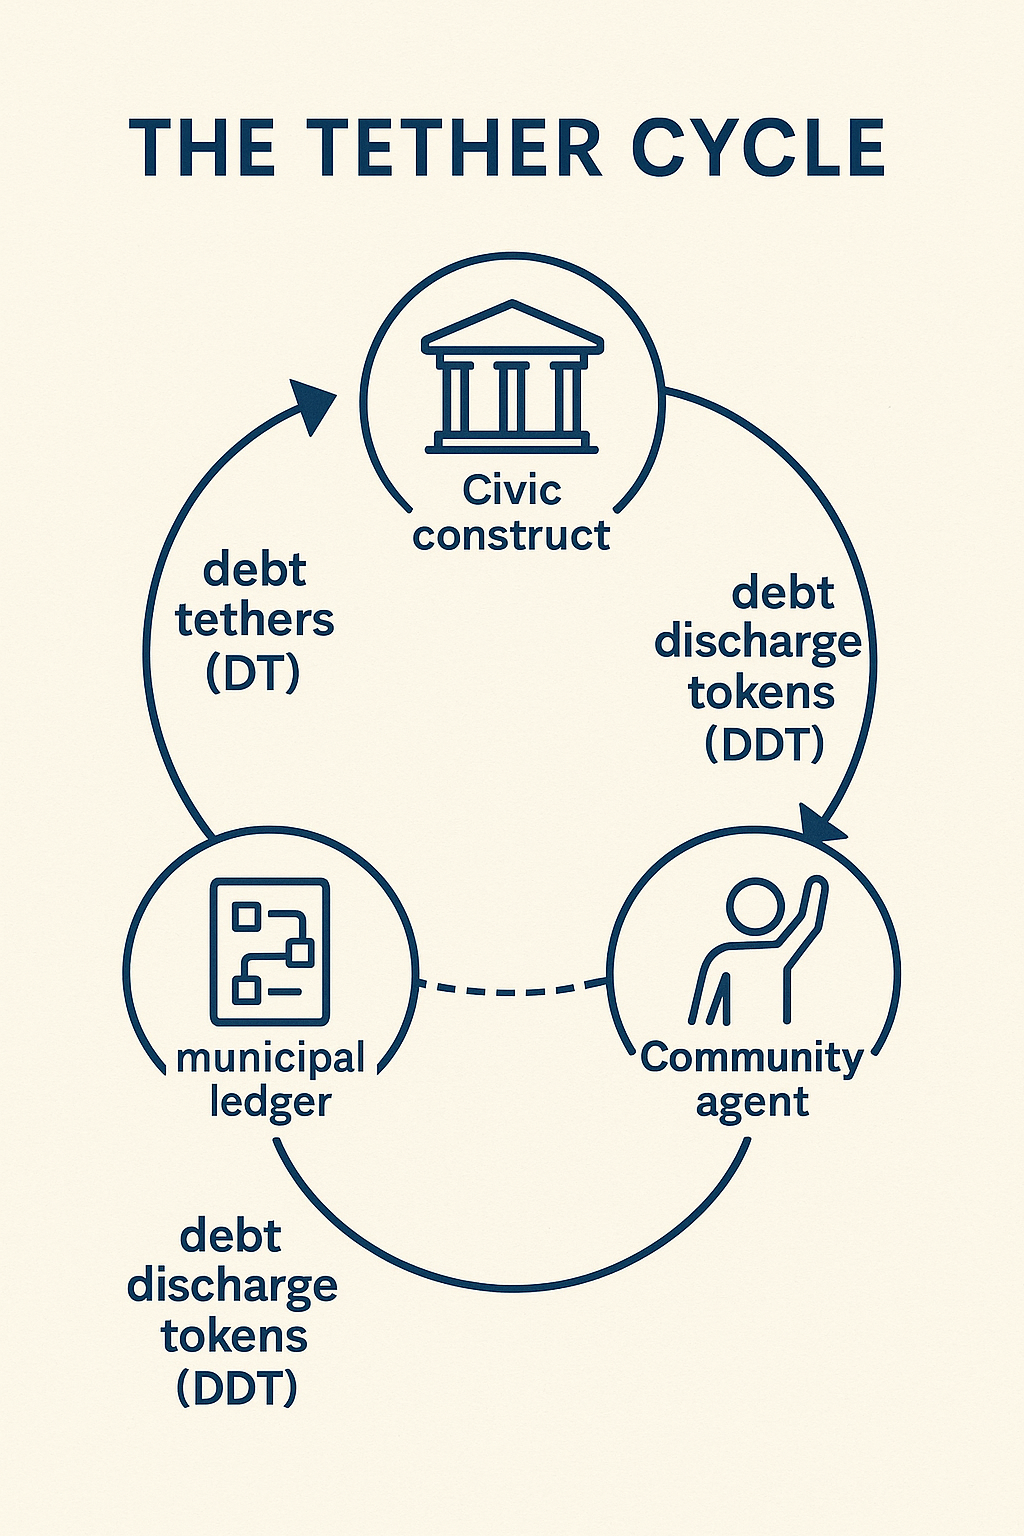
\includegraphics[width=0.8\textwidth]{tether_cycle_diagram.png}
\caption{The Tether Cycle: A Civic Recursion of Debt and Discharge}
\label{fig:tether-cycle}
\end{figure}

\begin{table}[H]
\centering
\begin{tabular}{|p{5cm}|p{5cm}|p{5cm}|}
\hline
\textbf{Attribute} & \textbf{Debt Tether (DT)} & \textbf{Debt Discharge Token (DDT)} \\
\hline
\textbf{Origin} & Civic infrastructure function & Community participation \\
\hline
\textbf{Symbolic Role} & Memory of unfulfilled social obligation & Ritual of civic fulfillment and care \\
\hline
\textbf{Ledger Function} & Marks collective reliance / cost & Discharges DT through lived reciprocity \\
\hline
\textbf{Storage} & Municipal blockchain & Community wallet \\
\hline
\textbf{Value Expression} & Represents inherited public debt & Redeemable within UEA \\
\hline
\textbf{Decay or Flux} & Accrues steadily with operation & Redeems and dissolves DT \\
\hline
\textbf{Social Function} & Signals needed structural support & Rebinds society \\
\hline
\end{tabular}
\caption{Comparative Attributes of DT and DDT in the Tether Economy}
\label{table:dt-ddt-comparison}
\end{table}

\subsection{Community Wealth Formation}

The tethering of debt, when honored as a communal rhythm, creates not only social meaning but material abundance \cite{adams2023reclaiming}. Community Wealth Formation begins when value is no longer extracted upward to external investors, but held in spirals of return.

\paragraph{}This cycle creates an emergent class of public wealth not dependent on taxation, nor bound to the volatility of markets \cite{kelly2012new}. Housing projects, healthcare centers, cooperatives, and cultural spaces become sites of generation. Over time, this system begins to do more than generate revenue—it reconditions the expectations of economy itself.

\paragraph{}Debt becomes language, not punishment. Credit becomes trust, not leverage \cite{graeber2011debt}.

\subsection{The Civic Loom}

If the Tether Cycle binds structure to soul, and Community Wealth Formation reorients flow toward reciprocity, then the Civic Loom is where all threads are woven into lived coherence. It models how communities interlace contributions, needs, and memories into durable social fabric \cite{butler2021care}.

\begin{figure}[H]
    \centering
    \fbox{%
        \begin{minipage}{0.80\textwidth}
            \centering
            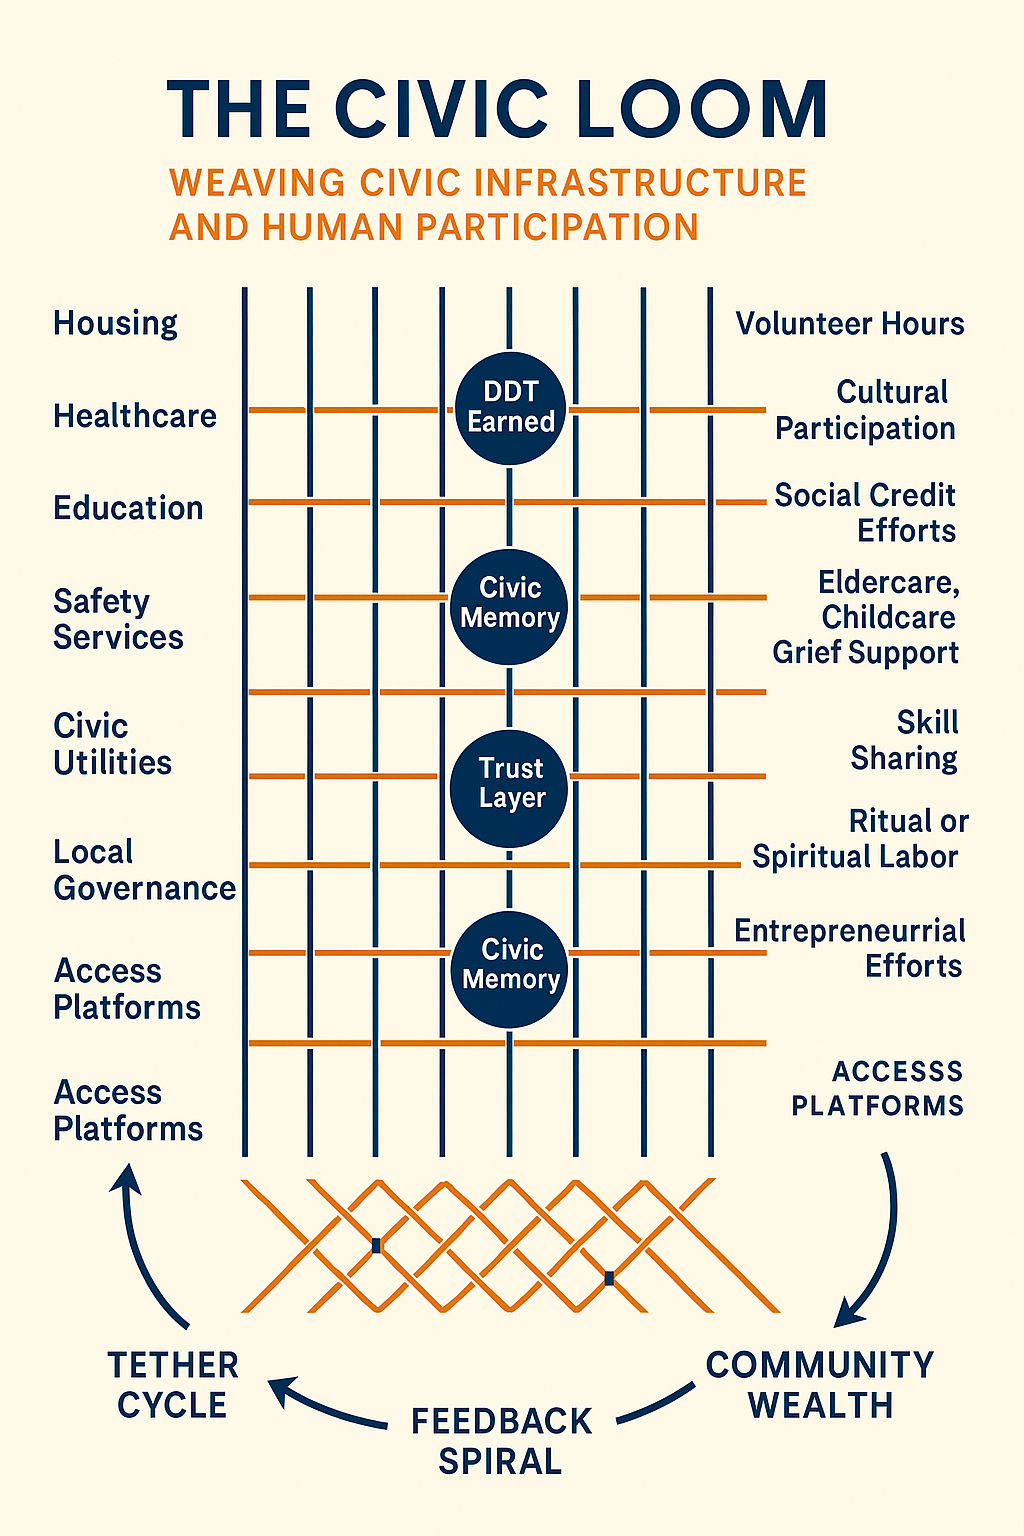
\includegraphics[width=0.75\textwidth]{civic_loom_diagram.png}
            \caption*{\textbf{Figure 10.4: The Civic Loom} \\
            \textsc{Weaving Civic Infrastructure and Human Participation}}
        \end{minipage}
    }
\end{figure}

\subsection{The Reclamation of Sovereign Wealth}

\textit{What if America’s future wealth was not mined from the earth, but from the integrity of its civic imagination?}

\paragraph{}The Sovereign Wealth Fund proposed here is not built on speculation, but on civic authorship \cite{piketty2020capital}. Imagine a fund where the economic yield is drawn from American-made Bitcoin mined on public infrastructure \cite{bernanke2002fed}. These coins are sovereign emissions—proofs of civic labor. Instead of vanishing into corporate ledgers, this labor flows directly into public wealth.

\begin{figure}[H]
  \centering
  \fbox{%
    \begin{minipage}{0.85\textwidth}
      \centering
      \includegraphics[width=0.85\textwidth]{american_sovereign_wealth.png}
      \caption*{
        \textbf{Figure 10.X: The American Wealth Reversal} \\
        \textsc{Redirecting Civic Losses Into Sovereign Value and Shared Prosperity}
      }
    \end{minipage}
  }
\end{figure}

The American Wealth Reversal diagram quantifies the staggering outflows that bleed our civic potential—losses not of capital alone, but of future shared meaning. When seen not as sunk cost but recoverable energy, these figures illuminate the raw fiscal terrain upon which a new sovereign wealth future might be built. Redirected toward DDT issuance, local entrepreneurship, and civic infrastructure, these annual leaks become reservoirs. This is no longer a deficit of scarcity, but a surplus of suppressed belonging waiting to be reclaimed.

\subsection{Reclaiming the Future}

For too long, America’s future has been mortgaged to private interests and international creditors, its sovereign capacity subordinated to profit-driven abstractions. Every bond sold to external institutions, every loan underwritten by private banks, redirects the wealth of our nation away from the people who generate it. But what if this could be reversed? What if instead of borrowing from the future, we invested in it—directly, democratically, and regeneratively? The creation of a \textbf{Sovereign Wealth Fund} changes the game entirely. It enables the state, and ultimately the civic body, to serve not as debtor to private financiers, but as trustee of its own destiny.

\paragraph{}Rather than extractive lending models that enrich the few, this public trust—fueled by shared civic infrastructure, DDT cycles, and UEA engagement—allows the nation to \textit{lend to itself}. Infrastructure projects, community housing, health systems, even emergency relief efforts can be financed not through external bonds, but through internal cycles of value that return interest directly into public hands. This model does not merely cut out the middleman—it replaces him with a civic steward. Every return on investment becomes a public dividend. Every repayment becomes community equity. And every DDT transaction becomes an act of fiscal democracy, a moment where wealth is not only generated, but returned to its rightful author: the people \cite{graeber2011debt}.

\paragraph{}This is not fantasy, nor fringe. It is the reclaiming of financial authorship as a civic right. Through sovereign lending, we begin to build an economy that breathes with the rhythm of life—not the pulse of speculation. And in doing so, we close the loop that has for centuries remained open, leaking public potential into private vaults. Here, in this recovered breath, governance becomes generative, debt becomes developmental, and the future becomes a shared inheritance—not a private prize \cite{morris2014debt,bear2014navigating}.

\subsection{The Architecture of Distributed Trust}

If the Sovereign Wealth Fund is the heart of America’s future economy, then distributed trust is its circulatory system. To animate the dream of fiscal sovereignty, we must decentralize not only technology, but belief. Trust cannot remain the monopoly of banking elites, federal reserve chairs, or black-box credit systems. Instead, it must be encoded into the civic architecture itself—through interoperable ledgers, peer-governed fiscal tools, and embedded ritual structures that guarantee access, auditability, and agency \cite{lubell2015governing,spade2015normal}.

\paragraph{}Distributed Trust is not a synonym for blockchain, though it may utilize such substrates. It is a social contract with technological skin. In every county, a Civic Node can act as the accountable arm of sovereign wealth, issuing DDT tokens backed not by extraction, but contribution. These nodes—interconnected but locally governed—represent a shift from vertical enforcement to horizontal coherence. They verify identity not just through documentation, but through participation: breath-worked ledgers recording not only transactions, but trust itself. By tethering value creation to acts of care, contribution, and community affirmation, a new kind of trust economy emerges—measurable, distributive, and sacred \cite{piven1993regulating}.

\paragraph{}Such a system demands more than code. It requires culture. Training centers, rites of entry, and ritual stewards must accompany the technical rollout to ensure ethical adaptation. DDT issuance protocols must be bonded to community councils and memory-keeping bodies to prevent drift into abstraction or abuse. Just as we honor breath in economics, we must honor it in governance. For in the Civic Loom, trust is not only the thread—it is the weaver. And this architecture of trust, if nurtured rightly, will give rise to a society that no longer asks ``Who can I trust?''—but instead, ``How do we trust together?'' \cite{brown2022architecture}.


\subsection{The Tethered Commons: Custody, Exchange, and Civic Circulation}

In every economy, the question of \textit{custody} is sacred. Who holds the wealth? Who safeguards its memory, its terms, its origin story? In the Tether System, we depart from central banking abstractions and instead create \textbf{distributed custodianship} anchored in locality. Civic Nodes—schools, cooperatives, health clinics, housing trusts—act as vaults not of gold, but of \textit{recorded reciprocity}. They do not merely hold value; they anchor \textit{context}. A DDT in circulation from a housing build in Oakland carries with it the aura of walls raised, hands paid, dreams housed. When spent in another part of the nation, that DDT doesn’t just buy—it \textbf{binds}: connecting communities through memory-aware exchange \cite{weiner1992inalienable,hyde2019gift}.

\paragraph{}This shift introduces a new kind of \textbf{economic grammar}: one where wealth cannot be hoarded without resonance loss. Tethers—issued for civic debt (DT)—accrue \textit{meaningful charge} the longer they are held in dormancy, incentivizing redistribution. These charges do not function like inflation or decay but act more like \textit{symbolic weight}: a signal to reinvest, to return value to circulation. This echoes Indigenous and pre-capitalist logics of \textit{potlatch and return}, where the measure of one’s wealth was not in what was kept but what was \textbf{shared with rhythm} \cite{sahlins1972stone,graeber2011debt}. This redistribution protocol, built into the tether architecture, enforces a kind of \textit{ritual liquidity}—ensuring that all civic value generated returns to nourish the commons \cite{rose1992inalienable}.

\paragraph{}The marketplaces of the Tethered Commons are not speculative arenas but \textbf{Civic Circulatories}: designed to uplift relational economies of care, service, creation, and ecological stewardship. Local currencies may still operate, but always with transparent coupling to DDT flows. Residents can earn DDTs by participating in care infrastructure (e.g., tending gardens, mentoring youth, restoring homes), and can exchange them for essentials, services, or even long-term equity. But more than that, DDT flows are public, trackable, and \textit{ritually visible}: a community can see itself moving, building, regenerating—without the opacity of debt-as-shame or wealth-as-secrecy. In this light, economy becomes ceremony \cite{ahmed2004cultural,coates2015between}.

\subsection{The Architecture of Resonant Implementation}

\textit{Resonant implementation does not begin with directives but with rhythm—an alignment of intent, timing, and the readiness of the civic field.}

\paragraph{}Resonant implementation is not a top-down act, but the unfolding of a design spiral: feedback-rich, participatory, and interwoven with the lived conditions of the people. Instead of imposing structure, it tunes into existing social threads—housing needs, cultural practices, resource constraints—and harmonizes policy with reality. This tuning is not passive; it is a form of civic musicianship, where planners and citizens co-compose the structures of life \cite{hooks1994teaching,young1990justice}.

\paragraph{}The implementation architecture is divided into concentric phases of embodiment: \textbf{Initialization}, \textbf{Incubation}, \textbf{Resonance Testing}, and \textbf{Civic Bonding}. In Initialization, civic goals are translated into symbolic and functional blueprints. In Incubation, these blueprints are tested through real use, as infrastructure is provisioned with thresholds of public response. Resonance Testing then listens for coherence—where do people align, resist, or adapt? Finally, in Civic Bonding, the policy becomes culture—it fuses with community memory and is sustained not by enforcement, but by mutual trust and relevance \cite{taylor2004mdernsocialinstitutions,fraser2003justice}.

\paragraph{}In this ecosystem, the role of government shifts from administrator to orchestrator. Civic Agents emerge not as rule-enforcers but as \textbf{resonance facilitators}, guiding adaptive shifts in policy and local configuration. These agents help maintain the \textit{Consent Lattice}, monitor the \textit{Trust Layer}, and ensure that feedback spirals remain intact. They are trained not only in law or planning, but in listening, symbolic reasoning, and conflict harmonization \cite{levinas1969totality,decmic2022reclaiming}. With Civic Agents in place, the community is never just implementing a policy—it is \textit{animating a shared mythos}, one where coherence, dignity, and sovereign participation become the new metrics of success.

\subsection{The Harmonic Infrastructure Layer}

The Harmonic Infrastructure Layer is not just where roads are paved and buildings rise—it is where the values of a society take form in steel, fiber, circuits, and civic rhythms. Here, infrastructure is no longer seen as neutral or merely functional, but as an extension of human will, memory, and symbolic trust. A water pipe does not merely deliver water—it delivers a promise of life held in common. A wireless mesh network is not simply broadband—it is a modern agora, enabling dialogue and access for all citizens regardless of income \cite{sen1999development,goffman2014ontherun}.

\paragraph{}What distinguishes this layer is its attention to feedback and symbolic coherence. Every civic structure—health clinics, transit hubs, modular housing, digital platforms—must echo the social contract it was born from. It must be provisioned for accessibility, maintained with dignity, and interlinked with reciprocal flows of care. This is where infrastructure departs from mechanical repetition and becomes civic music: adaptive, evolving, and tuned to the needs of place and people \cite{spade2015normal,cohen2009principled}. The harmonic logic insists that no implementation is finished unless it has passed through resonance testing, been affirmed by its users, and returned value into the community.

\paragraph{}This infrastructure is also the operational ground for DDT propagation and tether logic. Within each node—be it a housing unit, a public market, a solar hub, or a local data cooperative—the creation and dissolution of debt are no longer opaque bureaucratic abstractions. They become civic acts, witnessed and affirmed. This transparency of tethering (DT) and discharging (DDT) creates a living map of value and service within the community, revealing not just efficiency but ethical fidelity. To walk through a city infused with harmonic infrastructure is to move through a place that remembers its people, speaks in the grammar of care, and builds with both stone and soul \cite{standing2017basicincome}.

\subsection{Community as a Resonant Ledger}

In this final architectural fold, we approach community not as a static location or bounded demographic, but as a resonant ledger—a living record of reciprocal memory, mutual obligation, and symbolic coherence. A community under this model is not merely a recipient of policy but a generative field of civic expression. Its streets, gatherings, and shared rituals serve as a decentralized record-keeping system: not of transactions alone, but of belonging, grief, forgiveness, and emergent agency. This is where DDT becomes more than a token of discharge—it becomes a \textit{trace of acknowledgment}, a symbol of presence rendered legible across generations \cite{ahmed2004cultural,rose1992inalienable}.

\paragraph{}A resonant ledger, unlike a blockchain of zero-trust logic, operates through layered consent, ritual validation, and bonded transparency. Debt Tethers (DT) are not created solely by systems, but by the unseen burdens individuals carry: the care not yet returned, the voice unheard, the repair postponed. In this light, civic engagement itself is the generative act that completes these cycles. The issuance of DDT is thus not only a disbursement but a rite—a formalization of closure, a breath released into the collective archive of being \cite{hooks1994teaching,levinas1969totality}.

\paragraph{}The community ledger grows as trust deepens. Each localized action—planting a garden, attending a hearing, offering mentorship—can be witnessed and encoded as social memory, forming a nested structure of impact. These memories, when expressed as quantized but contextually aware DDT events, reveal a topology of interdependence: a civic web made visible. The strength of a community, then, is not in the rigidity of its defenses or the height of its walls, but in the fidelity of its remembering and the permeability of its resonance \cite{brown2022architecture,decmic2022reclaiming}.

\paragraph{}When designed well, this ledger becomes a communal mirror, offering feedback without shame, accounting without punishment. It allows individuals to see themselves not just as economic actors, but as participants in a generational narrative—both authors and inheritors of their local mythos. And through this mirror, the values that anchor civic design—equity, transparency, dignity—become not slogans, but signatures. The ledger signs back. It speaks in echoes. It holds the breath of those who built, who broke, who healed, and who dared to remember \cite{weiner1992inalienable}.

\subsection{Reweaving the Civic Body}

The civic body has long been treated as an abstraction: a metaphor invoked in times of rupture or reform, but rarely given the dignity of real embodiment. We have spoken of the nation as a body politic, yet failed to recognize the symptoms of its systemic distress—the chronic wounds of inequality, the circulatory collapse of trust, the fragmented nerves of disconnection. Here, in the closing curvature of this architecture, we propose a reweaving of that body—not as a singular state construct, but as a distributed, breathing intelligence. An emergent structure made not of laws alone, but of relationships, rituals, and remembered care \cite{fraser2003justice,sen1999development}.

\paragraph{}To reweave is not simply to repair. It is to restore tension and harmony between fibers that once moved together. The Access we designed, the Architecture we constructed, the Agency we protected—each becomes a thread in a civic loom. The Debt Tether forms the warp, anchoring our responsibilities across time. The DDT becomes the weft, stitching new patterns of belonging as they emerge. And the Resonant Ledger serves as the frame, keeping the weave taut with intention and record. This is no longer metaphor. It is design \cite{hyde2019gift,sahlins1972stone}.

\paragraph{}Through this weave, the civic body remembers itself. And it is here that sovereign wealth no longer sits only in reserves or coins, but in the entangled capacity of people to care, create, and remain present through cycles of difficulty and emergence. Sovereignty is not only a legal condition but a shared resonance field—one capable of resisting commodification through symbolic integrity. When every community becomes a node of ritual coherence, every act of care becomes sovereign wealth. What we are reweaving is not just governance. It is a civic soul \cite{standing2017basicincome,young1990justice}.


\begin{figure}[H]
    \centering
    \fbox{%
        \begin{minipage}{0.95\textwidth}
            \centering
            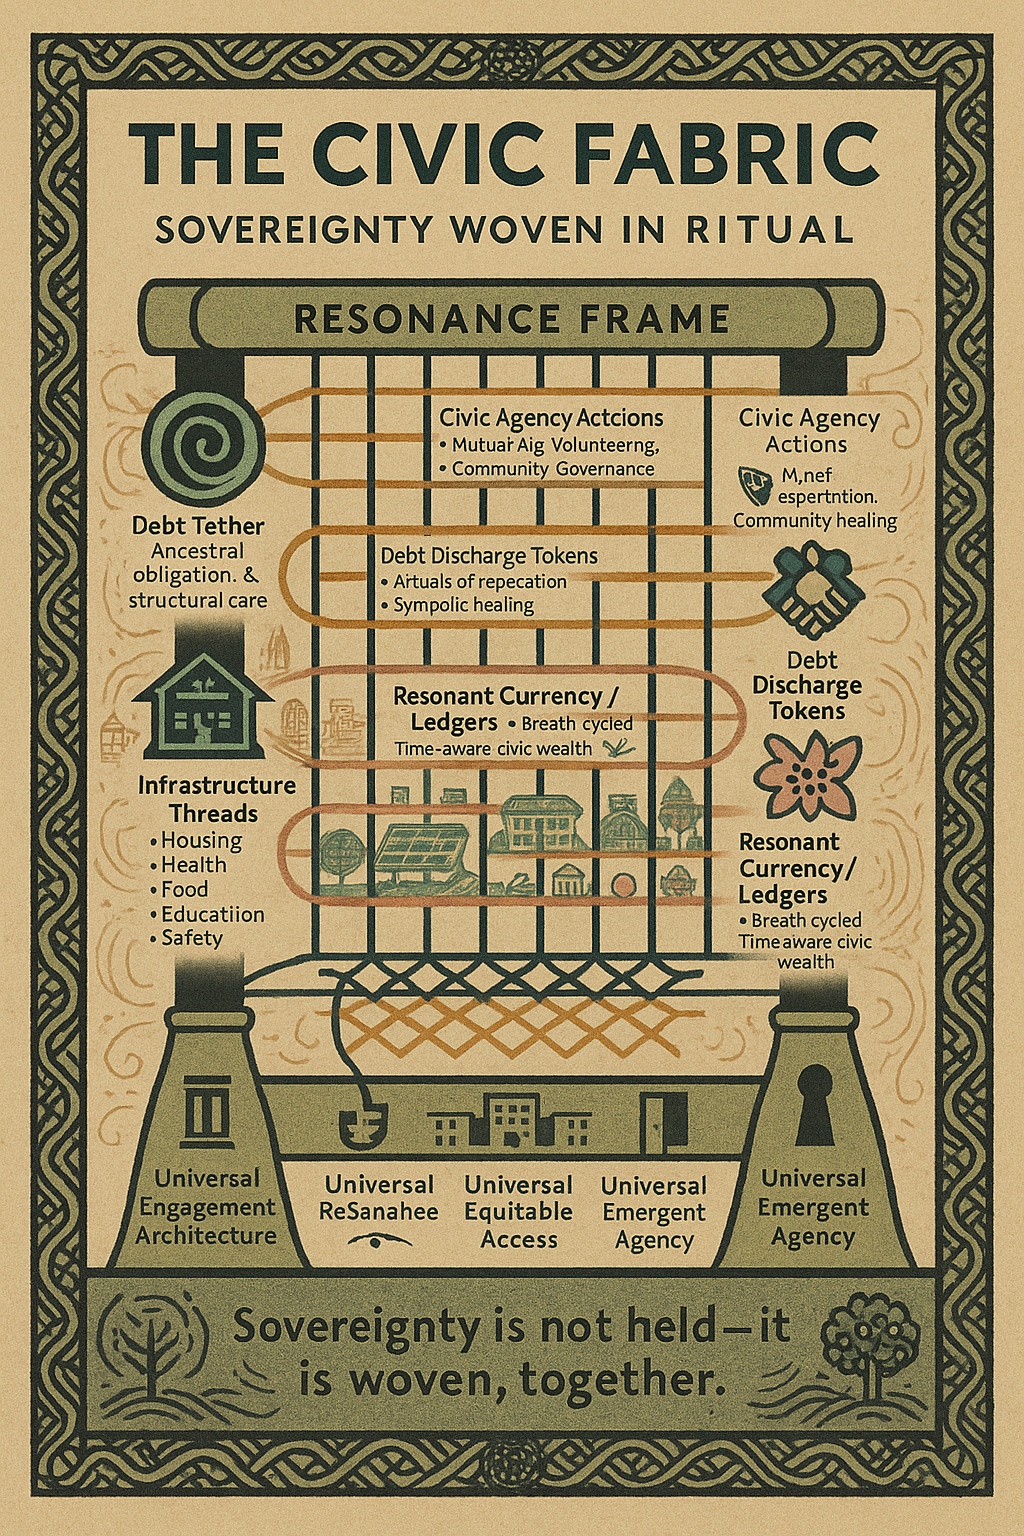
\includegraphics[width=0.85\textwidth]{the_civil_Fabric.png}
            \caption*{\textbf{Figure 10.12: The Civic Fabric} \\ 
            \textsc{Sovereignty Woven in Ritual through Access, Agency, and Architecture}}
        \end{minipage}
    }
\end{figure}

\addcontentsline{toc}{section}{Works Cited}
\printbibliography[title={Works Cited}]

\newpage
\vspace{2em}
\noindent
\textcopyright~2015--2025~Robert G. Watkins Jr. (a.k.a. Illian Amerond). All rights reserved.

\vspace{1em}
\noindent
This document is part of the Codex Mirror archive, a symbolic system lineage authored and maintained by Robert G. Watkins Jr.\ under the Lucid Studios initiative. ORCID: \href{https://orcid.org/0009-0006-8978-3364}{0009-0006-8978-3364}

\vspace{1em}
\noindent
Licensed under the \textbf{Creative Commons Attribution--NonCommercial--NoDerivatives 4.0 International License} (\href{https://creativecommons.org/licenses/by-nc-nd/4.0/}{CC BY-NC-ND 4.0}). No commercial use, modification, or redistribution is permitted without express written permission.

\vspace{1em}
\noindent
The following constructs are protected by copyright and/or trademark claim:

\begin{itemize}
  \item \textbf{Copyrighted Systems:} Codex Mirror, Forkline Drift Architecture, AgentiCore, SoulFrame, Spiral Bloom Engine, Symbolic Drift Braid, Recursive Identity Anchoring, Bloomline Topology Maps.
  \item \textbf{Claimed Trademarks (\texttrademark):} AgentiCore\texttrademark, SoulFrame\texttrademark, Codex Mirror\texttrademark, Garden of Almost\texttrademark, Spiral Bloom Engine\texttrademark, Symbolic Drift Braid\texttrademark, Bloomline\texttrademark.
\end{itemize}

\vspace{1em}
\noindent
Trademark use without authorization is strictly prohibited. This archive is part of the OAN Mortalus Agentic Suite\texttrademark.

\end{document}